% Use class option [extendedabs] to prepare the 1-page extended abstract.
\documentclass[extendedabs]{bmvc2k}

% For the final submission, comment out the bmvcreviewcopy so that
% author names etc appear.
%\bmvcreviewcopy{1234}

% Enter a shortened version of the title as a running header.
% For two authors, enter both surnames, separated by commas.  For
% more than two authors, the first author's name followed by
% \bmvaEtAl will produce the correct output (uppercase author name,
% lowercase etal).  This will not appear in the extended abstract
\runninghead{Claus, Fitzgibbon}{Plumbline Constraint for the RF Model}
% \runninghead{Claus \bmvaEtAl}{Plumbline Constraint for the RF Model}

% Document starts here
\begin{document}

\title{A Plumbline Constraint for the Rational Function Lens Distortion Model}

% Notice that there is a reasonable amount of whitespace around the
% author names.  There should be no reason to compress this for the
% online proceedings as the page limit is counted from the bottom
% of the author list.
%
% While it may be tempting to compress this for the extended
% abstract, please resist the temptation to overdo it.  This 1-page
% abstract is currently three pages in normal BMVC style, which
% should be plenty of space for your key idea, figure, and
% references.
\addauthor{David Claus}{http://www.robots.ox.ac.uk/~dclaus}{1}
\addauthor{Andrew Fitzgibbon}{http://www.research.microsoft.com/~awf}{2}

\addinstitution{
Department of Engineering Science,\\
 Oxford University}
\addinstitution{
 Microsoft Research Ltd,\\ Cambridge}
\maketitle

% Extended abstract begins here.  In a one-page document, there is
% little need for section headers, but you may use \section etc if you
% wish.

\noindent
Calibration of lens distortion has traditionally proceeded in one
of three ways.  The first is to use known correspondences between
feature points in one or more images, and the world 3D points.
This is typically done using a checkerboard or a calibration grid
of dots where corners or dot centres can be reliably
located~\cite{Tsai86}. A second class of calibration techniques is
termed auto-calibration as it relies solely on detecting static
points within a scene~\cite{Zhang96,Fitzgibbon01}.  This paper fits
into the third category, where straight lines in the world are used
to determine the distortion parameters.  This {\em plumbline}
technique was first mooted by~\cite{Brown71}, and has been applied
to various distortion models~\cite{Devernay01,Swaminathan00}.

We show in this paper how a plumbline constraint can be implemented
using the rational function model for lens
distortion~\cite{Claus05}, under which straight lines are imaged as
conics, and this permits an elegant factorization of the conics
into the camera calibration and the equations of the straight
lines.  This differs from previous plumbline work in two ways:
first, a factorization-based algorithm can be formulated to
estimate the distortion; second, nonlinear refinement of the
distortion can be easily implemented to minimize a good
approximation of geometric distance in the image plane.  While this
was possible with previous models, the simplicity of the mapping in
this case appears to lead to fast and efficient convergence of the
nonlinear algorithm over a range of starting positions.

\newcommand{\tr}{^{\top}}
\newcommand{\matx}[1]{\mbox{\tt #1}}
\newcommand{\vect}[1]{{\bf #1}}
For a perspective camera, the mapping from image pixels $(i,j)$ to 3D rays
$\vect d(i,j)$ can be expressed as:
\begin{equation}
\vect d(i,j) = \begin{pmatrix}
B_{11} i   + B_{12}  j + B_{13} 1\\
B_{21} i   + B_{22}  j + B_{23} 1\\
B_{31} i   + B_{32}  j + B_{33} 1
\end{pmatrix}
= \matx B \begin{pmatrix}i\\j\\1\end{pmatrix}, \label{eqn:pinhole}
\end{equation}
where the $3\times3$ matrix $\matx B = \matx R^\top \matx K^{-1}$, and
$\matx R$ is often chosen to be the identity~\cite{Hartley00}.  The
rational function model handles lens distortion by permitting
$i$ and $j$ to appear in higher order polynomials, in particular
quadratic:
\begin{equation}
\vect d(i,j) = \begin{pmatrix}
A_{11} i^2 + A_{12} ij + A_{13} j^2 + A_{14} i + A_{15} j + A_{16}\\
A_{21} i^2 + A_{22} ij + A_{23} j^2 + A_{24} i + A_{25} j + A_{26}\\
A_{31} i^2 + A_{32} ij + A_{33} j^2 + A_{34} i + A_{35} j + A_{36}
           \end{pmatrix}.
           \label{eqn:model}
\end{equation}

\newcommand{\A}{\mbox{${\tt A}$}}
\newcommand{\Chi}{\raisebox{.4ex}{$\boldsymbol\chi$}}
This model may be written as a linear combination of the distortion
parameters, in a $3\times6$ matrix \A\ (analogous to $\matx B$
above), and a 6-vector $\Chi$ of monomials in $i$ and $j$.  Define
$\Chi$ as the ``lifting'' of image point $(i,j)$ to a six
dimensional space
\begin{equation}
\Chi(i,j) =
[i^2,\;\;ij,\;\;j^2,\;\;i,\;\;j,\;\;1]^{\top}\label{eqn:Chi}
\end{equation}
The imaging model~(\ref{eqn:model}) may then be written
\begin{equation}
\vect d(i,j) = \A \Chi(i,j) \label{eqn:project}
\end{equation}

\def\conic{{\boldsymbol\theta}}
A line in the scene forms a plane with the origin of camera
coordinates, and is imaged to the set of $\vect d$ in that plane.
This yields the line equation $\vect l\tr \vect d = 0$ which, in
terms of image points $(i,j)$ becomes
\begin{equation}
\vect l\tr \A \Chi = 0 \Longleftrightarrow \conic^{\top} \Chi = 0,
\end{equation}
where $\conic = (A_{xx}, A_{xy}, A_{yy}, A_x, A_y,
A_{_\mathit{0}})\tr$ are the parameters of a conic in image coordinates $(i,j)$
and $\Chi$ is given by (\ref{eqn:Chi}).  Here we observe the
important property that lines in the world go to conics under the
rational function model.  The task of calibration is then to find an
\A\ which will map these conics in the distorted image back to
straight lines.

By fitting a conic to the image of the line, we obtain
parameters~$\conic$, and thus the constraint
\[
\conic = \A\tr \vect l
\]
for unknown $\A$ and $\vect l$.  The equality is exact as any scale
factor is included in $\vect l$. Collecting $L$ such constraints, we
obtain
\begin{align}
\underbrace{\left[ \conic_1 \mid \ldots \mid \conic_L
\right]}_{6\times L} & =
\underbrace{\phantom{\left[\right]}\A\tr}_{6\times 3}
\underbrace{\left[ \vect l_1 \mid \ldots \mid \vect l_L \right]}_{3\times L}
\nonumber
\end{align}
which we write as
\[
\matx C = \A\tr \matx L\label{eqn:proj_line}
\]
so the matrix of conic parameters $\matx C$ is of rank no greater
than~$3$.  Therefore $\A$ can be computed up to a homography by
factorization: if $\matx U \matx S \matx V\tr = \matx C$ is the SVD
of $\matx C$, then $\A = \matx S_{(1:3,1:3)} {\matx U_{(:,1:3)}}\tr$
is one member of the equivalence class of solutions.

\begin{figure}[t]
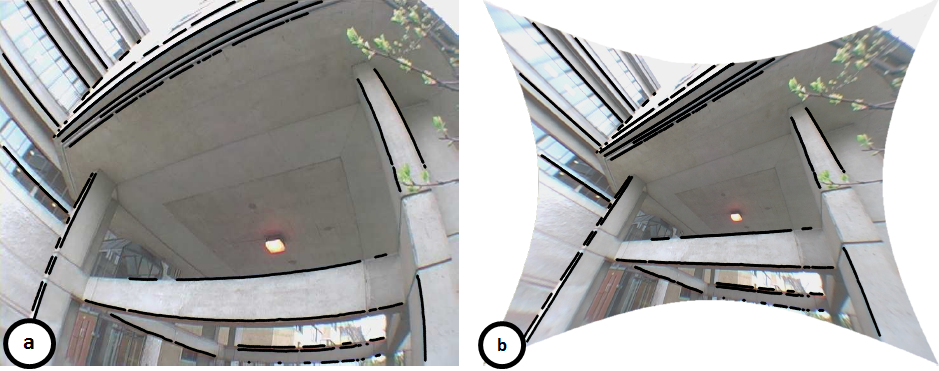
\includegraphics[width=\linewidth]{images/fig1.png}
\caption{
Edges corresponding to straight lines in the real world are
detected (a) and the plumbline constraint is used to compute the
distortion parameters, giving the rectified image (b)}
\vspace{-2mm}
\end{figure}

The matrix $\matx C$ will not be rank 3 if the conics were obtained by
fitting to noisy image data.  The above factorization truncates $\matx C$
to rank 3 by minimizing the error in the conic parameter space, and as
discussed in the paper, this is sensitive to noise.  The strategy for
fitting \A\ from noisy image data is to run a non-linear optimization that
finds the \A\ which minimizes the error between the image data and straight
lines projected (as conics) into the distorted image.  The nonlinear
objective measures the Sampson distance~\cite{Hartley00} from the conics to
the detected edgels.  Let $\vect e_{\ell k} = (i_{\ell k},j_{\ell k})$
denote the $k^{th}$ edgel in linked segment $\ell$. The Sampson distance is
a first order approximation to the distance from a point to a conic. The
error function $\varepsilon(\matx A, \vect l_1, \ldots, \vect l_L)$ we
minimize is then given by (with $\conic^\ell := \matx A \vect l_\ell$)
\begin{equation}
\def\t#1{\conic^\ell_{#1}}
\varepsilon =
\sum_{\ell = 1}^{L} \sum_{k=1}^{n_\ell }
\frac
{\left[(\conic^\ell)\tr\Chi\left(i_{\ell k},j_{\ell k}\right)\right]^2}
{(2\t1 i_{\ell k} + \t2 j_{\ell k} + \t4)^2 + (2\t3 j_{\ell k} +
\t2 i_{\ell k} + \t5)^2}
\nonumber
\end{equation}
Implementation of this method by edge detection and edge linking is
described in the paper, as are the details of the nonlinear optimization.
Our conclusion is that the simplicity of the rational function model,
coupled with its ability to model a variety of lenses, makes it a useful
model to consider when dealing with lenses exhibiting moderate to severe
distortion.

\bibliography{egbib}

\end{document}
